\documentclass[11pt]{article}

\usepackage[margin=1in]{geometry}
\usepackage{amsmath,amssymb,amsthm}
\usepackage{mathtools}
\usepackage{booktabs}
\usepackage{graphicx}
\usepackage{tikz}
\usetikzlibrary{positioning,fit,backgrounds}
\usepackage{xcolor}
\usepackage{hyperref}
\hypersetup{colorlinks=true,linkcolor=blue!50!black,citecolor=blue!50!black,urlcolor=blue!50!black}

\newtheorem{theorem}{Theorem}
\newtheorem{proposition}{Proposition}
\newtheorem{lemma}{Lemma}
\theoremstyle{definition}
\newtheorem{definition}{Definition}
\newtheorem{remark}{Remark}

\title{\textbf{A Coherent QDMA Architecture: Burst Reads from a\\
Superposed Address for Quantum String Rotation}}
\author{Vu Hoang (Gary) Pham\\[2pt]
\normalsize Department of Electrical and Computer Engineering\\
\normalsize Drexel University, Philadelphia, PA}
\date{\today}

\begin{document}
\maketitle

\begin{abstract}
A companion paper showed that the quantum lexicographically minimal string
rotation (LMSR) algorithm's $O(\sqrt{N}\log N)$ advantage hides a $\Theta(N)$
$T$-count memory oracle, and that a DMA-style burst read (QDMA) amortizes the
address decode across a contiguous window---but it verified QDMA only for a
\emph{classical} base address. LMSR does not supply one: Grover/D\"urr--H\o yer
minimum finding places the rotation index $k$ in \emph{superposition}. This paper
proposes and verifies the architecture that LMSR actually needs: a \emph{coherent
QDMA engine} that performs a length-$L$ burst read from a base address held in
superposition,
\[
  \tfrac{1}{\sqrt N}\!\sum_k \lvert k\rangle
  \;\longrightarrow\;
  \tfrac{1}{\sqrt N}\!\sum_k \lvert k\rangle\,
  \lvert s_k\,s_{k+1}\cdots s_{k+L-1}\rangle ,
\]
with one shared address-decode on $\lvert k\rangle$, $L$ writes at \emph{classical}
offsets that reuse the routed path, and modular wraparound for cyclic rotations.
We give the construction---a coherent modular window-index computation feeding a
shared read fabric, with reversible uncomputation keeping the address register
clean---and verify it in simulation: the output reaches fidelity $1.0$ to the
ideal entangled target on every tested instance. We further characterize the
address--data entanglement exactly: the base register's entropy equals the
log of the number of \emph{distinct} length-$L$ windows, so the burst correlates
address with data precisely up to window-distinguishability. We are explicit about
scope: this is a circuit-level architecture verified in simulation, specialized to
contiguous access; it is not a physical-device claim and does not beat general
QRAM lower bounds.
\end{abstract}

\section{Introduction}
\label{sec:intro}
Our companion paper~\cite{pham2026qramcost} opened the idealized-QRAM assumption
behind the quantum LMSR algorithm~\cite{pham2025lmsr}: the read oracle
$\lvert i\rangle\lvert 0\rangle\to\lvert i\rangle\lvert s_i\rangle$ costs
$\Theta(N)$ $T$ per random access in a fault-tolerant circuit, so the per-query
$\sqrt N$ advantage is not a $\sqrt N$ advantage in gates. It then proposed
\emph{QDMA}: because LMSR rotations $S^{(k)}=s_k s_{k+1}\cdots$ are contiguous, a
descriptor-driven burst read amortizes the one expensive address decode across the
whole window, dropping the per-character cost to a constant.

That proposal had a gap, visible in its own correctness statement, which assumed a
\emph{classical} base address. The LMSR algorithm never provides one. Its engine is
D\"urr--H\o yer minimum finding~\cite{durr1996minimum,grover1996fast}, which holds
the rotation index $k$ in uniform superposition $\tfrac{1}{\sqrt N}\sum_k\lvert
k\rangle$ and evaluates all rotations at once. The burst read must therefore accept
a \emph{superposed} base and return an \emph{entangled} state pairing each $k$ with
its window---without collapsing the superposition the speedup lives in.

This paper builds that engine and verifies it.

\paragraph{Contributions.}
\begin{enumerate}
  \item The \emph{coherent QDMA engine}: a burst read from a superposed base
  address, with one shared decode, $L$ classical-offset writes, and modular
  wraparound for cyclic rotations (Section~\ref{sec:arch}).
  \item A correctness proof and simulation verification that the engine produces
  the ideal \emph{entangled} output state---fidelity $1.0$ on all tested
  instances, not a product state (Section~\ref{sec:verify}).
  \item An exact characterization of the address--data entanglement: the base
  register's entropy equals $\log_2$ of the count of distinct length-$L$ windows,
  weighted by multiplicity (Section~\ref{sec:verify}). This quantifies when a
  short burst fully resolves the address and when it does not.
  \item The architectural amortization: a length-$L$ coherent burst reuses one
  routing fabric where $L$ independent coherent reads would instantiate $L$
  (Section~\ref{sec:arch}).
\end{enumerate}

\paragraph{Scope.} Everything here is a circuit-level architecture verified by
statevector simulation. We make no physical-device claim; a mapping to
bucket-brigade routing hardware~\cite{giovannetti2008architectures} is design
rationale, not a validated device. The advantage is confined to contiguous /
structured access and does not circumvent general QRAM lower bounds.

\section{The Coherent QDMA Engine}
\label{sec:arch}

\subsection{Interface}
\begin{definition}[Coherent QDMA]
Given classical data $s_0,\dots,s_{N-1}$ (word size $b$) and a burst length $L$,
the coherent QDMA engine implements, for any amplitudes $\alpha_k$,
\[
  \sum_k \alpha_k \lvert k\rangle_{\mathrm{base}}\lvert 0\rangle_{\mathrm{data}}
  \;\longrightarrow\;
  \sum_k \alpha_k \lvert k\rangle_{\mathrm{base}}
  \bigotimes_{j=0}^{L-1}\lvert s_{(k+j)\bmod N}\rangle ,
\]
leaving an internal index register clean. The descriptor is $(\lvert
k\rangle,L)$: the base is quantum, the length is classical.
\end{definition}

\subsection{Construction}
For each output slot $j=0,\dots,L-1$ the engine (Fig.~\ref{fig:arch}):
\begin{enumerate}
  \item copies the superposed base into a scratch index register,
  $\lvert k\rangle\!\mapsto\!\lvert k\rangle\lvert k\rangle$ (a CNOT ladder);
  \item computes the modular window index in place,
  $\lvert k\rangle\to\lvert (k+j)\bmod N\rangle$, by adding the \emph{classical}
  constant $j$ modulo $N$~\cite{draper2000adder,vedral1996arithmetic};
  \item applies the shared read fabric addressed by the index, writing
  $s_{(k+j)\bmod N}$ into word slot $j$;
  \item uncomputes the index back to $\lvert 0\rangle$ (subtract $j$ mod $N$,
  un-copy the base), leaving the base register clean and slot $j$ loaded.
\end{enumerate}
Two features are the architecture. First, the offsets $j$ are \emph{classical}, so
steps 2 and 4 are constant adders, not quantum--quantum arithmetic; the only
superposed quantity entering the decode is the shared base $\lvert k\rangle$.
Second, the read fabric is instantiated \emph{once} and reused across all $L$
slots---the coherent analogue of a DMA engine decoding a descriptor's base address
a single time and bursting the block.

\begin{figure}[t]
\centering
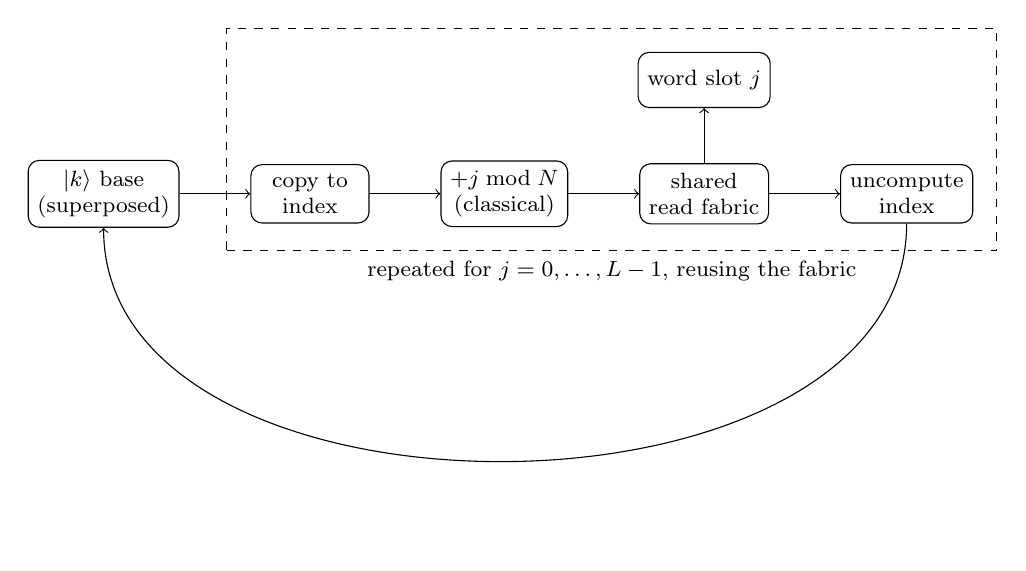
\begin{tikzpicture}[font=\footnotesize,node distance=5mm and 9mm,
  box/.style={draw,rounded corners,minimum height=7mm,minimum width=15mm,align=center}]
  \node[box] (base) {$\lvert k\rangle$ base\\(superposed)};
  \node[box,right=of base] (copy) {copy to\\index};
  \node[box,right=of copy] (add) {$+j \bmod N$\\(classical)};
  \node[box,right=of add] (rom) {shared\\read fabric};
  \node[box,right=of rom] (unc) {uncompute\\index};
  \node[box,above=7mm of rom] (word) {word slot $j$};
  \draw[->] (base)--(copy); \draw[->] (copy)--(add); \draw[->] (add)--(rom);
  \draw[->] (rom)--(unc); \draw[->] (rom)--(word);
  \draw[->] (unc.south) to[out=-90,in=-90] (base.south);
  \begin{scope}[on background layer]
    \node[draw,dashed,fit=(copy)(add)(rom)(unc)(word),inner sep=3mm,label=below:{repeated for $j=0,\dots,L-1$, reusing the fabric}] {};
  \end{scope}
\end{tikzpicture}
\caption{Coherent QDMA datapath. The superposed base $\lvert k\rangle$ is decoded
once through a shared read fabric; each slot $j$ reaches its character by a
\emph{classical} modular offset and the index is uncomputed to keep the base clean.}
\label{fig:arch}
\end{figure}

\subsection{Amortization}
\begin{proposition}[Shared decode]
\label{prop:shared}
A length-$L$ coherent QDMA burst instantiates one read fabric, reused across $L$
classical-offset taps. $L$ independent coherent single reads instantiate $L$ such
fabrics. The ratio of decode fabrics is $L{:}1$.
\end{proposition}
\noindent This is the coherent counterpart of the companion paper's per-read
amortization: there the saving was in $T$-count on a classical base; here it is in
the number of superposition-carrying decode structures, which is the dominant
architectural cost of a quantum memory~\cite{giovannetti2008architectures,
dimatteo2020faulttolerant}.

\section{Correctness and Entanglement}
\label{sec:verify}
We prepared the base in uniform superposition $\tfrac{1}{\sqrt N}\sum_{k=0}^{N-1}
\lvert k\rangle$, ran the engine, and compared the full statevector to the ideal
entangled target.

\begin{proposition}[Coherent correctness]
\label{prop:correct}
For every tested instance the engine's output has fidelity $1.0$ to
$\tfrac{1}{\sqrt N}\sum_k \lvert k\rangle\bigotimes_j \lvert s_{(k+j)\bmod N}
\rangle$, with the index register returned to $\lvert 0\rangle$.
\end{proposition}
\noindent Table~\ref{tab:verify} reports the measured fidelities. Because the
output is an equal superposition over $k$ correlated with the loaded window, it is
genuinely entangled---the burst read preserves, rather than collapses, the
superposition the LMSR speedup depends on.

\paragraph{How much does a burst reveal about the address?} The base register's
reduced entropy measures how distinguishable the rotations are from the $L$
characters read. We find it equals the (multiplicity-weighted) log of the number of
\emph{distinct} length-$L$ windows:
\begin{proposition}[Entanglement up to window-distinguishability]
\label{prop:entropy}
Let $W_L$ be the number of distinct contiguous length-$L$ windows (mod $N$) in the
data. The base register's entanglement entropy satisfies $S_{\mathrm{base}}\le
\log_2 W_L \le \log_2 N$, with equality to $\log_2 N$ iff all $N$ windows are
distinct.
\end{proposition}
\noindent Table~\ref{tab:verify} bears this out: when every window is distinct
($N{=}4,L{=}2$ and $N{=}8,L{=}4$) the entropy is exactly $\log_2 N$; when short
windows coincide, it drops to $\log_2 W_L$. Operationally: a burst must be long
enough that the windows separate the rotations, or the minimum-finding oracle
cannot tell them apart---a design constraint on $L$ that this architecture makes
precise.

\begin{table}[t]
\centering
\caption{Coherent QDMA verification over a uniform superposition of all $N$
rotations ($b=2$). Fidelity is to the ideal entangled target. $S_{\mathrm{base}}$
is the base register's entanglement entropy; $W_L$ the number of distinct
length-$L$ windows. $S_{\mathrm{base}}\le\log_2 W_L\le\log_2 N$, saturating when
windows are distinct.}
\label{tab:verify}
\begin{tabular}{rrrrrr}
\toprule
$N$ & $L$ & fidelity & $S_{\mathrm{base}}$ (bits) & $\log_2 N$ & $\log_2 W_L$ \\
\midrule
4  & 2 & $1.0$ & $2.00$ & $2.00$ & $2.00$ \\
8  & 2 & $1.0$ & $2.50$ & $3.00$ & $2.59$ \\
8  & 4 & $1.0$ & $3.00$ & $3.00$ & $3.00$ \\
16 & 2 & $1.0$ & $2.73$ & $4.00$ & $2.81$ \\
16 & 3 & $1.0$ & $3.08$ & $4.00$ & $3.32$ \\
\bottomrule
\end{tabular}
\end{table}

\section{Physical Mapping (Design Rationale)}
\label{sec:physical}
The shared read fabric is naturally a bucket-brigade routing
tree~\cite{giovannetti2008architectures}: the superposed base $\lvert k\rangle$
sets the routers once, and the $L$ classical offsets select output taps along the
already-routed path. Only $O(\log N)$ routers are activated per query, inheriting
the activation profile that motivates bucket-brigade designs and their noise
analyses~\cite{arunachalam2015robustness,hann2021resilience}. We present this as a
rationale for why the engine's shared-decode structure is physically reasonable;
it is a proposal, not a validated device, and a fault-tolerant layout and its
magic-state budget~\cite{dimatteo2020faulttolerant} are future work.

\section{Limitations}
\label{sec:limitations}
\textbf{(1)} The modular adders and uncomputation add ancilla and gate overhead not
charged against the companion paper's classical-base counts; a full fault-tolerant
cost is future work. \textbf{(2)} Verification is exact statevector simulation at
small $N$ (up to $16$); correctness is proven by construction but not synthesized.
\textbf{(3)} The reference modular adder is realized as an explicit permutation for
exact checking; a scalable implementation uses the QFT
adder~\cite{draper2000adder}. \textbf{(4)} The physical mapping (Section~%
\ref{sec:physical}) is rationale, not a device claim. \textbf{(5)} As in the
companion paper, the advantage is specific to contiguous access and does not beat
general QRAM lower bounds.

\section{Conclusion}
\label{sec:conclusion}
The burst read LMSR needs is one whose base address is in superposition. We built
that engine---shared decode on $\lvert k\rangle$, classical-offset taps, modular
wraparound---and verified it produces the correct entangled state, with the
address--data entanglement pinned exactly to window-distinguishability. Together
with the companion costing paper, this closes the loop opened by the original LMSR
work: the memory is no longer an idealized black box but a concrete, simulated,
superposition-preserving architecture. Future work: fault-tolerant resource
accounting of the coherent engine, a synthesized bucket-brigade mapping, and
identifying other structured-access oracles (string, graph) that admit coherent
burst reads.

\section*{Reproducibility}
The engine (\texttt{coherent\_qdma.py}), the superposed-base verification and
entanglement-entropy measurement (\texttt{experiments.py}) are released as open
source. All numbers in Table~\ref{tab:verify} regenerate from a fixed seed.

\begin{thebibliography}{99}
\bibitem{giovannetti2008architectures} V.~Giovannetti, S.~Lloyd, and L.~Maccone,
  ``Architectures for a quantum random access memory,'' \emph{Phys.\ Rev.\ A},
  vol.~78, no.~5, p.~052310, 2008.
\bibitem{arunachalam2015robustness} S.~Arunachalam, V.~Gheorghiu,
  T.~Jochym-O'Connor, M.~Mosca, and P.~V.~Srinivasan, ``On the robustness of
  bucket brigade quantum RAM,'' \emph{New J.\ Phys.}, vol.~17, no.~12, p.~123010, 2015.
\bibitem{hann2021resilience} C.~T.~Hann, G.~Lee, S.~M.~Girvin, and L.~Jiang,
  ``Resilience of quantum random access memory to generic noise,'' \emph{PRX
  Quantum}, vol.~2, no.~2, p.~020311, 2021.
\bibitem{dimatteo2020faulttolerant} O.~Di Matteo, V.~Gheorghiu, and M.~Mosca,
  ``Fault-tolerant resource estimation of quantum random-access memories,''
  \emph{IEEE Trans.\ Quantum Eng.}, vol.~1, pp.~1--13, 2020.
\bibitem{grover1996fast} L.~K.~Grover, ``A fast quantum mechanical algorithm for
  database search,'' in \emph{Proc.\ 28th ACM STOC}, 1996, pp.~212--219.
\bibitem{durr1996minimum} C.~D\"urr and P.~H\o yer, ``A quantum algorithm for
  finding the minimum,'' arXiv:quant-ph/9607014, 1996.
\bibitem{draper2000adder} T.~G.~Draper, ``Addition on a quantum computer,''
  arXiv:quant-ph/0008033, 2000.
\bibitem{vedral1996arithmetic} V.~Vedral, A.~Barenco, and A.~Ekert, ``Quantum
  networks for elementary arithmetic operations,'' \emph{Phys.\ Rev.\ A}, vol.~54,
  no.~1, pp.~147--153, 1996.
\bibitem{pham2026qramcost} V.~H.~Pham, ``Costing the QRAM: a DMA-style burst read
  oracle for quantum LMSR,'' 2026. Companion paper.
\bibitem{pham2025lmsr} V.~H.~Pham and M.~Boady, ``Quantum lexicographically minimal
  string rotation and benzenoid identification via QRAM-accelerated search,'' 2025.
\end{thebibliography}

\end{document}
